% Template for ICASSP-2010 paper; to be used with:
%          mlspconf.sty  - ICASSP/ICIP LaTeX style file adapted for MLSP, and
%          IEEEbib.bst - IEEE bibliography style file.
% --------------------------------------------------------------------------
\documentclass{article}
\bibliographystyle{plain}

% use Times
\usepackage{times}
% For figures
\usepackage{graphicx} % more modern
%\usepackage{epsfig} % less modern
\usepackage{subfigure} 
% For algorithms
\usepackage{algorithm}
\usepackage{algorithmic}

% As of 2011, we use the hyperref package to produce hyperlinks in the
% resulting PDF.  If this breaks your system, please commend out the
% following usepackage line and replace \usepackage{icml2014} with
% \usepackage[nohyperref]{icml2014} above.
\usepackage{hyperref}

% Packages hyperref and algorithmic misbehave sometimes.  We can fix
% this with the following command.
\newcommand{\theHalgorithm}{\arabic{algorithm}}

\usepackage{color}
\usepackage{amsthm}
\usepackage{amsmath}
\usepackage{amsfonts}

\newtheorem{theo}{Theorem}
\newtheorem{prop}[theo]{Proposition}
\newtheorem{lemm}[theo]{Lemma}
\newtheorem{prof}[theo]{Proof}
\renewcommand{\theprof}{}

  
\DeclareMathOperator{\rch}{RCH_\eta}
\DeclareMathOperator{\ch}{CH}
\DeclareMathOperator{\argmin}{argmin}
\DeclareMathOperator{\argmax}{argmax}
\newcommand{\re}{\mathbb{R}}
\newcommand{\na}{\mathbb{N}}
\newcommand{\rand}{{\rm Random}}
\newcommand{\randre}{{\rm RandomReal}}
\newcommand{\red}{\mathbb{R}^d}
\newcommand{\bi}{\left\lbrace -1,1 \right\rbrace}
\newcommand{\m}{{\rm minimize}}
\newcommand{\M}{{\rm maximize}}
\newcommand{\st}{{\rm subject~ to}}
\newcommand{\ms}{R_\ominus}
\newcommand{\me}{E_\ominus }
\newcommand{\aff}{{\rm aff} }


\newcommand{\emptyValue}{
empty value: This is the value of $C$.
%empty value: This is the $C$ in the function above.
%This value is created as ${\rm Rand(max-min)+min}$.
%We can select the range of value $f(\emptyset)$.
%The left side is the minimum value and the right side is the maximum value.
%The min value is inclusive but the maximum value is exclusive (i.e. [min..max)).
%The range, the minimum value and the maximum value must be within signed $32$-bit integer.
%It is possible that ${\rm min}={\rm max}$.
%In this case, the application only returns the minimum value.
}

\newcommand{\modular}{modular: This is the value of $m$.
%This value is created as created empty value above.
}

\newcommand{\exTab}[1]{
In the #1 tab,
the application creates datasets for making such submodular functions.}

\newcommand{\out}[1]{
Let $n$ be the cardinality of the ground set.
Then, output files have $#1$ lines as follows.\\ \mbox{}\\
}



%\address{
\begin{document}
%\fontsize{9pt}{10.8pt}\selectfont
\fontsize{10pt}{12pt}\selectfont
%\ninept
%

\title{How to Use Submodular Dataset Creator }
\author{onigiri}
\date{\today}


\maketitle
\newpage


\tableofcontents

\newpage

\section{Introductions}
This is the document for Submodular Dataset Creator.
We recommend you to read \ref{commonLeftSec}, \ref{allSec} and 


\section{Common Usage of Left Side}\label{commonLeftSec}
We will explain how to use functions on the left side of the application,
which are common in any tabs.

\begin{figure*}[h!]\label{commonPic}
{
\fontsize{10pt}{12pt}\selectfont
\centering
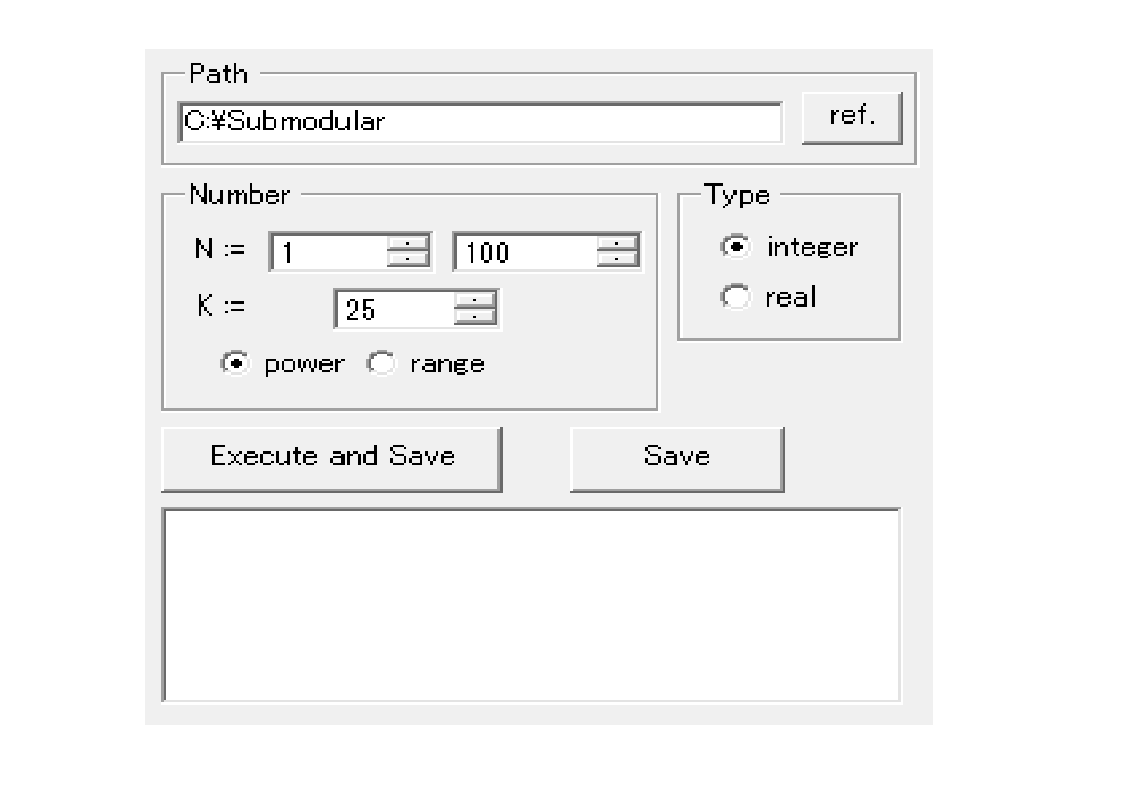
\includegraphics[height=7.0cm]{picture/CommonFunction.png}
\caption{Common Functions}
}
\end{figure*}

\subsection{Path}\label{pathSec}
We need to select a path in order to decide where we save data.
You can directly type the path or select it by clicking "ref." button.
If you type the path and it does not exist,
new folder is automatically created.

\subsection{Number}\label{numberSec}
We can select $N$ and $K$,
where $N$ is the cardinality of ground sets
and $K$ is the number of datasets for each cardinality.
The application create datasets like Algorithm \ref{alg:for}.
Here, $N_{\min}$ is the blank on left side of $N$
and $N_{\max}$ is the one on right side.
If we choose "power", ${\sf Increment(i)}=2*i$,
and if we choose "range", ${\sf Increment(i)}=i+1$.
For example, in the Figure \ref*{commonPic},
The application makes $25 ~ (=K)$ datasets whose cardinality of the ground sets are $1,2,4,8,16,32$ and $64 ~ (=N)$.



\begin{algorithm}[h!]
\fontsize{10pt}{12.0pt}\selectfont
   \caption{"Create Datasets"}
   \label{alg:for}
\begin{algorithmic}
   \FOR{($i=N_{\min}$; $i\leq N_{\max}$; $i= {\sf Increment(i)}$)}
   \FOR{($j=0$; $j<K$; $j++$)}
   \STATE Create a dataset whose the cardinality of the ground set is $i$.
   \ENDFOR
   \ENDFOR
\end{algorithmic}
\end{algorithm}

\subsection{Type}\label{typeSec}
\textcolor{red}{To be Written!!!}


\subsection{Execute and Save}
The application make datasets as stead in subsection \ref{pathSec}, \ref{numberSec} and \ref{typeSec},
and save something as stead in subsection \ref{saveSec}.
The files are created as ${\rm path}/{\rm tabname}/n\_k$,
where ${\rm path}$ is set in subsection \ref{pathSec},
${\rm tabname}$ is the name of tab which is currently selected (except All tab),
$n$ is the cardinality of the ground set
and $k$ is the index of the dataset.


\subsection{Save}\label{saveSec}
\textcolor{red}{To be Written!!!}

\subsection{Text Box}
In the bottom on the left side, there exist a text box.
If the application haves some trouble or 
it executes something,
logs are output on this text box.


\newpage


\section{Common Usage of Right Side}\label{commonRightSec}
We will explain how to use functions on the right side of the application,
which are common in any tabs expect the All tab.

\subsection{Range Blank}
\begin{figure*}[h!]\label{rangeFormPic}
{
\fontsize{10pt}{12pt}\selectfont
\centering
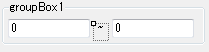
\includegraphics[height=2.0cm]{picture/rangeForm.png}
\caption{Range Blank}
}
\end{figure*}
We first explain how to select a range of a random value.
In order to select the range,
you need to set two values, a minimum value and a maximum value.
The left blank is for minimum value ($\min$)
and the right blank is for maximum value ($\max$).
Then, the range is defined by $[\min..\max]$ (inclusive and inclusive) if the type is integer
and $[\min..\max)$ (inclusive and exclusive) if the type is real (See \ref{typeSec} for the type).

From the definition above,
if the type is real and $\min=\max$,
then $[\min..\max)$ has no range.
Therefore, it seems that $\min=\max$ is not allowed.
However, for convenience, the application always returns $\min (=\max)$ in this case.


\subsection{Value Blank}
We next explain value blank.
The range blank has two blanks but value blank has only one blank.
If you type a value in the blank,
then this value is set as the parameter.

\begin{figure*}[h!]\label{valueFormPic}
{
\fontsize{10pt}{12pt}\selectfont
\centering
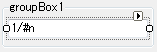
\includegraphics[height=2.0cm]{picture/valueForm.png}
\caption{Value Blank}
}
\end{figure*}

\subsection{Use Variable in a Blank}
You can use variable $n$, where $n$ is the cardinality of the ground set.
For example, if you want to set the value as $1/n$,
please type $1/\#n$ or $1/\#N$.
If the value should be integer but the calculated value is not integer,
this value is rounded down.

\newpage

\section{All}\label{allSec}

\begin{figure*}[h!]\label{allPic}
{
\fontsize{10pt}{12pt}\selectfont
\centering
\includegraphics[height=7.0cm]{picture/all.png}
\caption{Candidates of datasets}
}
\end{figure*}
In All tab,
the application creates datasets which are checked at a time.
There for if you want to make data with same condition,
it is very useful.
For the parameters on the left side of the application, like $N,K,{\rm path}$, 
the application uses the ones of the All's tab,
but for the other parameters it uses the ones of each dataset's tab.

\newpage

\section{Undirected Cut}\label{undirectedCutSec}
Let $G=(V,E,w)$ be a complete undirected nonnegative weighted graph,
$\delta_w :V\rightarrow \re_{\geq 0}$ be an undirected weighted cut function,
$m$ be a modular function.
Then, $\delta_w + m$ is a submodular function.
\exTab{Undirected Cut}

We explain meanings of blanks in this tab.
\begin{itemize}
\item \modular
\item edge weight: This is the value of $w$.
This value must be non-negative.
In order to express $w$,
the application makes a symmetric matrix.
The $(i,j)$th entries of this matrix means that the weight of the edge from $i$ to $j$.
The application sets $(i,i)$th entries are $0$.
\end{itemize}
\out{2n+1}
$n$ \\
$m_1$ \\
$\vdots$ \\
$m_n$ \\
$w_{11}  \cdots w_{1n}$ \\
\mbox{\quad \quad}$\vdots$ \\
$w_{n1} \cdots w_{nn}$ \\


Here, $w_{i1}\cdots w_{in}$ is separated by an empty character " ".


\newpage

\section{Directed Cut}\label{directedCutSec}
Let $G=(V,E,w)$ be a complete directed nonnegative weighted graph,
$\delta_w :V\rightarrow \re_{\geq 0}$ be a directed weighted cut function,
$m$ be a modular function.
Then, $\delta_w + m $ is a submodular function.
\exTab{Directed Cut}
\begin{itemize}
\item \modular
\item edge weight: This is the value of $w$.
This value must be non-negative.
In order to express $w$,
the application makes a matrix.
The $(i,j)$th entries of this matrix means that the weight of the edge from $i$ to $j$.
The application sets $(i,i)$th entries are $0$.
\end{itemize}

\out{2n+1}
$n$ \\
$m_1$ \\
$\vdots$ \\
$m_n$ \\
$w_{11}  \cdots w_{1n}$ \\
\mbox{\quad \quad}$\vdots$ \\
$w_{n1} \cdots w_{nn}$ \\

Here, $w_{i1}\cdots w_{in}$ is separated by an empty character " ".


\newpage

\section{Connected Detachment}\label{connectedDetachmentSec}
See \cite{nash85} for details.
Let $G=(V,E)$ be a connected undirected graph,
$m$ be a modular function.
For all $X\subseteq V$,
let $c(X)$ be the number of connected component of induced subgraph $G(X)$
and $e(X)$ be the number of edges which is incident with $X$.
Then, $m(X)-e(X)+c(V\setminus X)-1$ is a submodular function.
\exTab{Connected Detachment}
\begin{itemize}
\item \modular
\item probability of edge: This is the probability $p$ that an edges exists.
The application makes random graphs with this $p$.
%In order to do that, we need a probability $p$.
%Of course $p$ must satisfy $0\leq p \leq 1$.
For each $(i,j)$ with $i+1<j$,
the application connects $i$ and $j$ if and only if ${\rm RandDobule}([0..1))<p$.
Note that since the graph is connected, it connects $i$ and $i+1$ in advance.
\end{itemize}

\begin{figure*}[h!]\label{adjListPic}
{
\fontsize{10pt}{12pt}\selectfont
\centering
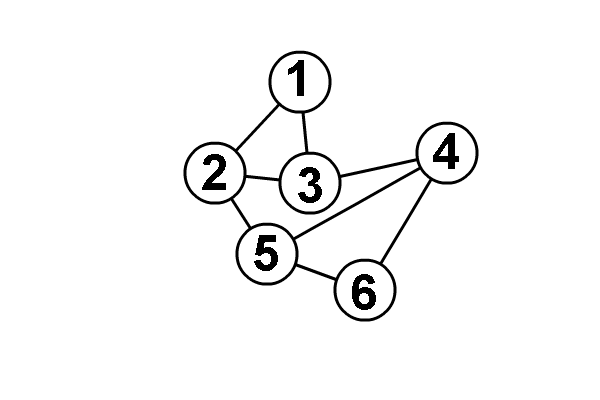
\includegraphics[height=7.0cm]{picture/graph.png}
\caption{example graph }
}
\end{figure*}

\out{2n+1}
$n$\\
$m_1$ \\
$\vdots$ \\
$m_n$ \\
$l_1e_{11}\cdots e_{1l_1}$\\
\mbox{\quad \quad}$\vdots$ \\
$l_ne_{n1} \cdots e_{nl_n}$ \\




Here, $l_i$ is the number of edges with incident with $i$,
and each element is separated by empty character " ".
Therefore, the graph is expressed by an adjacency list.


For example, if we are given a graph like \ref{adjListPic},
then the graph part of the output is as follows.
\mbox{}\\
\mbox{}\\
2 3\\
1 3 5\\
1 2 4\\
3 5 6\\
2 4 6\\
4 5\\


\newpage

\section{Facility Location}\label{facilityLocationSec}
Let $M\in \re^{n\times n}$ be a nonnegative matrix,
$m$ be a modular function.
Let $V:=\{1,\cdots n\}$.
For any $X\subseteq V$,
define 
\[
f(X) := m(X)   + \sum_{i\in V} \max \{M_{ij} \mid j\in X \}  \nonumber
\]
Then, $f$ is a submodular function.
\exTab{Facility Location}

\begin{itemize}
\item \modular
\item matrix element: This is the value of $M$.
\end{itemize}

\out{2n+1}
$n$\\
$m_1$ \\
$\vdots$ \\
$m_n$ \\
$M_{11}\cdots M_{1n}$\\
\mbox{\quad \quad}$\vdots$ \\
$M_{n1} \cdots M_{nn}$ \\


\newpage

\section{Graphic Matroid}\label{graphicMatroidSec}
Let $G=(V,E)$ be a graph.
For all $X\subseteq E$,
define $r(X):=\max \{ |Y| \mid Y\subseteq X, {\rm the~induced~subgraph~G(Y)~does~not~have~a~cycle.} \}$.
This $r$ is called the rank function of the graphic matroid which arises from $G$,
and therefore $r$ is a submodular function.
For example,
if $G$ is a graph showed in Figure \ref{garMatPic} then
$r(\{ \{1,3\},\{2,3\} \})=2$ and $r(\{ \{2,5\},\{4,5\},\{4,6\},\{5,6\} \})=3$.
Let $m$ be a modular function.
For all $X\subseteq V$,
define $f(X):=r(X)+r(V\setminus X)$.
Then, $f$ is also a submodular function.
\exTab{Graphic Matroid}

\begin{figure*}[h!]\label{garMatPic}
{
\fontsize{10pt}{12pt}\selectfont
\centering
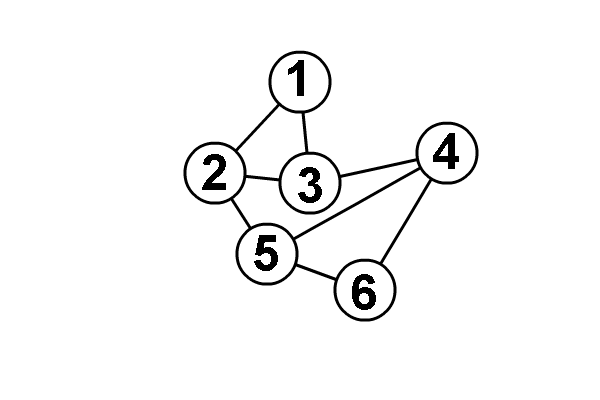
\includegraphics[height=7.0cm]{picture/graph.png}
\caption{example graph }
}
\end{figure*}

\begin{algorithm}[h!]
\fontsize{10pt}{12.0pt}\selectfont
   \caption{"Create $n$ edges"}
   \label{alg:nEdges}
\begin{algorithmic}
   \FOR{($i=1$; $i\leq n$; $i= i+1$)}
   \STATE $u_i:= {\rm Rand}(|V|)$
   \STATE $v_i:= {\rm Rand}(|V|)$
   \STATE connect $u$ and $v$
   \ENDFOR
\end{algorithmic}
\end{algorithm}

\begin{itemize}
\item \modular
\item number of vertices:
This is $|V|$.
Let this value is $n$.
Then the application uses Algorithm \ref{alg:nEdges} to make $n$ edges.

\end{itemize}

\out{2n+2}\\
$n$\\
$m_1$ \\
$\vdots$ \\
$m_n$ \\
$|V|$ \\
$u_1~v_1$\\
\mbox{}~~~ $\vdots$\\
$u_n~v_n$\\

Here, $|V|$ is the number of vertices
and $u_i$ and $v_i$ is the ones described in Algorithm \ref{alg:nEdges}.





\newpage

\section{Binary Matrix Rank}\label{binaryMatirxRankSec}
Let $M^0,M^1 \in \re^{k\times n}$ be a binary matrix,
i.e., a matrix whose elements are $0$ or $1$,
and $V:=\{1,2,\cdots ,n\}$.
Denote the $i$th column vector of the matrix $M$ by $M_i$.
For all $X\subseteq V$,
define $r(X):= \max \{ |Y| \mid Y\subseteq X, (M_i)_{i\in Y} {\rm is~linearly~independent.} \}$.
Then, $r$ is the rank function of $M$ according to column,
and it is a submodular function.
Let $m$ be a modular function.
For all $X\subseteq V$,
define $f(X):=m(X)+r(X)+r(V\setminus X)$.
Then, $f$ is also a submodular function.
\exTab{Binaray Matrix Rank}

\begin{itemize}
\item \modular
\item probability of element: This is the probability of the $(i,j)$th element is $1$
(and the others are $0$).
\item column length: This is $k$ above.

\end{itemize}

\out{n+k+2}
$n$\\
$m_1$ \\
$\vdots$ \\
$m_n$ \\
$k$ \\
$M_{11}\cdots M_{1n}$\\
\mbox{\quad \quad}$\vdots$ \\
$M_{k1} \cdots M_{kn}$ \\


\newpage

\section{Negative Symmetric Matrix Summation}\label{NegativeSymmetricMatrixSummationSec}
Let $M\in \re_{\leq 0 }^{n\times n}$ be a symmetric matrix whose elements are non-positive,
$V:=\{1,2,\cdots,n\}$,
$m$ be a modular function.
For all $X\subseteq V$,
define $f(X):=m(X)+\sum_{i,j\in X}M_{ij}$.
Then, $f$ is a submodular function.
\exTab{Negative Symmetric Matrix Summation}

\begin{itemize}
\item \modular
\item matrix element: This is the value of $M$.
This value must be non-positive.
\end{itemize}

\out{2n+1}
$n$\\
$m_1$ \\
$\vdots$ \\
$m_n$ \\
$M_{11}\cdots M_{1n}$\\
\mbox{\quad \quad}$\vdots$ \\
$M_{n1} \cdots M_{nn}$ \\


\newpage

\section{Set Cover}\label{setCoverSec}
Let $G=(V,U,E)$ be a bipartite graph with $|V|$,
$m_V$ be a modular function on $V$,
$m_U$ be a non-negative modular function on $U$
and $C$ be a constant.
For all $X\subseteq V$,
define $f(X):=m_V(X)+\varphi(N(X))$ is a submodular function.
Here, $N$ is a neighbor function, i.e.,
for all $X\subseteq V$, $N(X):=\{u \in U \mid \exists v\in X~ \{ u,v\}\in E  \} $
and $\varphi$ is a concave function.
\exTab{Set Cover}

\begin{itemize}
\item modular: This is the value of the modular function on $V$.
\item the cardinality of vertices: This is $|V|$.
\item weight of element: This is the value of the modular function on $U$.
This value is must be non-negative.
\item matrix element: This is the probability $p$ that an edge exists.
For each $(i,j)$ where $i\in V,j\in U$,
the application connects $i$ and $j$ if and only if ${\rm RandDobule}([0..1))<p$.
See Algorithm \ref{alg:randEdges} for details.
\end{itemize}


\begin{algorithm}[h!]
\fontsize{10pt}{12.0pt}\selectfont
   \caption{"Create random edges"}
   \label{alg:randEdges}
\begin{algorithmic}
   \REQUIRE{$p$ is the probability}
   \FOR{($i=1$; $i\leq |V|$; $i= i+1$)}
   \FOR{($j=1$; $j\leq |U|$; $j= j+1$)}
   \IF{ $\randre() < p$}	
   \STATE connect $i\in V$ and $j\in U$
   \ENDIF
   \ENDFOR
   \ENDFOR
\end{algorithmic}
\end{algorithm}

\out{3n+2}
$n$\\
$m_{V_{1}}$ \\
$\vdots$ \\
$m_{V_{n}}$ \\
$|U|$ \\
$m_{U_{1}}$ \\
$\vdots$ \\
$m_{U_{|U|}}$ \\
$l_1e_{11}\cdots e_{1l_1}$\\
\mbox{\quad \quad}$\vdots$ \\
$l_ne_{n1} \cdots e_{nl_n}$ \\

Here, $l_i$ is the number of edges with incident with $i$,
and each element is separated by empty character " ".
Therefore, the graph is expressed by an adjacency list.




\newpage




\bibliography{document.bib}


\end{document} 
